\documentclass{article}
\usepackage{leftidx}
\usepackage{hyperref}
\usepackage{caption}
\usepackage{subcaption}
\usepackage[utf8]{inputenc}
\usepackage[margin=1in]{geometry}
\hypersetup{
    colorlinks=true,
    linkcolor=blue,
    filecolor=magenta,      
    urlcolor=cyan,
}
\title{518 - Assignment 1}
\author{Bharti Mehta, Victor Zhang}
\date{March 22, 2021}

\usepackage[utf8]{inputenc}
\usepackage{amsmath}
\usepackage{amsfonts}
\usepackage{natbib}
\usepackage{graphicx}
% \usepackage{changepage}
\usepackage{amssymb}
\usepackage{xfrac}
% \usepackage{bm}
% \usepackage{empheq}
\usepackage{tikz}
\usepackage{dirtytalk}

\newcommand{\contra}{\raisebox{\depth}{\#}}

\newenvironment{myindentpar}[1]
  {\begin{list}{}
          {\setlength{\leftmargin}{#1}}
          \item[]
  }
  {\end{list}}

\pagestyle{empty}

\begin{document}

\maketitle
% \begin{center}
% {\huge Econ 482 \hspace{0.5cm} HW 3}\
% {\Large \textbf{Victor Zhang}}\
% {\Large February 18, 2020}
% \end{center}

\section{Introduction}
The purpose of this assignment was to create a scheduler to expose \verb|pthread|-like functionality via user threads. Our solution assumes that we are given one kernel thread and unlimited space within which to develop scheduling and multithreading. If the user is allowed to mix kernel and user threads, scheduling would become intractably difficult, since we have no control over how or when kernel threads run.

\section{Library Operation}
\subsection{Timing and Scheduler Concurrency}
The core scheduler relies on signals sent by an alarm \verb|timer| to run scheduling events.
\verb|SIGALRM| invokes \verb|schedule()|, which swaps threads and will be discussed later in this section.
Immediately, interrupt signals introduce thorny concurrency issues.
What happens if \verb|schedule| is called while we're in the middle of another scheduling decision?
Luckily, the signal handler blocks the same signal while executing, so we need not worry about interrupting while swapping.
Further, since we assume a single-threaded process, we may \say{enter} the scheduler by disarming the timer and \say{exit} the scheduler by re-arming the timer.
This gives us exclusive control of the process while scheduler-specific queues and other data are being accessed.
In particular, \verb|pthread| functions that require sequential access to important data structures call \verb|enter_scheduler()| like a user program would acquire a lock.

The \verb|schedule()| function handles swapping and is called by \verb|pthread| function to finish execution.
It is responsible for swapping out the currently running thread (front of the currently running queue), aging, and decay.
Finally, it invokes \verb|swapcontext| to run a new context.
The particulars of swapping will be discussed in a later section.

\subsection{Priority, Aging, and Decay}
Priority values can be assigned from \verb|0| to \verb|4|, inclusive.
Lower numbers indicate higher priority.
Each thread is allocated runtime based on priority:
% $$\mathrm{runtime} = 2^{\mathrm{priority}}$$
% For instance, a thread with priority \verb|3| will run for 8 continuous scheduling cycles.
$$\mathtt{runtime} = {\mathtt{priority}} + 1$$
For instance, a thread with priority \verb|3| will run for 4 continuous scheduling cycles.

Every thread starts with priority \verb|0|. 
Whenever \verb|schedule| is called within a thread's context, it ages according to the following algorithm:
\begin{itemize}
\item If \verb|schedule| is called via \verb|yield|, the priority does not change.
\item If the thread has run for its entire time slice, the priority is incremented by 1, up to \verb|MAX|.
\end{itemize}

A maintenance cycle is requested every second. We scan through the queues and reassign priority based formula
\begin{gather*}
\mathtt{new\_prio} = \left\lfloor (\mathtt{old\_prio}+1) \cdot e^{-x/g(\mathtt{old\_prio+1})} \right\rfloor\\
g(y) = \frac{\mathtt{CYCLES\_SINCE\_LAST}}{\ln y} - 1
\end{gather*}
$\mathtt{old\_prio} \in [1,\mathtt{MAX}]$ is the old priority of the thread. It makes no sense to decay threads with priority \verb|0| so we don't bother. $x \in [1,\infty)$ is the number of scheduling cycles since the thread was last run. \verb|CYCLES_SINCE_LAST| is the number of scheduling cycles since the last maintenance cycle.
This is an efficient way of ensuring older threads are not starved out of resources. Decay is faster for the lowest priority threads than higher priority threads. The parameters are set up so that threads which have run recently are not decayed, regardless of priority, but every thread is guaranteed to enjoy the highest priority if it has not been run since the last maintenance cycle.

\subsection{Swapping}
We maintain an array of linkedlist queues and a hashmap.
The hashmap is indexed by thread \verb|id| and contains information about all threads created in the process, alive or dead.
We implement multilevel priority queuing with the queue array.
Upon thread creation, we generate a \verb|tcb| for it containing a unique thread \verb|id|, context, and metadata for priority and joining threads.
We put the \verb|tcb| onto the back of the highest priority queue and into the hashmap.
We insert new threads onto the back of the queue to prevent starvation.
If we were to insert to the front, an adversary could starve old threads by continually creating new threads that run for only one scheduling cycle.

When the scheduler is invoked, it first checks the priority of the currently running thread.
If the thread has run for fewer contiguous cycles than its priority specifies, the scheduler exits, allowing the thread to run for longer.
If instead the thread indicates it intends to \verb|yield|, we move to the next step.
The currently running thread is placed at the back of the appropriate queue determined by the aging algorithm.
If a maintenance cycle is deemed necessary, it runs at this point.
Finally, we pick the highest priority ready thread to run.

\subsection{Priority Inversion}
In order to determine if a lower priority thread has acquired a lock while there exist higher priority threads waiting on the lock creating a priority inversion, we included a variable called \verb|hoisted_priority| for each lock. This variable is initially set to be an impossibly low priority, and is updated to match the priority of any thread which calls \verb|my_pthread_mutex_lock()| and has a higher priority than \verb|hoisted_priority|. In this way, we store the highest thread priority amongst those threads either waiting on or holding the lock. If a thread acquires the lock or is already holding it, we check if it has a lower priority than the \verb|hoisted_priority|. If it does, we ``hoist" the thread to the priority of the highest priority blocked thread, the \verb|hoisted_priority|. In this way, the owner of the lock will run before any other threads waiting on that lock, therefore avoiding a priority inversion. 

If a thread which acquires the lock needs no hoisting, in other words when an acquiring thread's priority is the same as \verb|hoisted_priority|, we know there are no blocked threads with a higher priority than the holding thread and so there cannot be a priority inversion at the moment. As a result, we reset \verb|hoisted_priority| to the impossibly low priority to ensure accurate priority inversion detection hereafter. 

\section{Testing and Analysis}

\subsection{Testing}
To test our thread library against the POSIX thread library, we measured the CPU time it took for each library to run the same program. For each library, the context spawning the threads called \verb|clock()| right before creating any attributes, locks, and threads, and right after joining with spawned threads and destroying any locks or attributes. In this way, we obtained the number of clock ticks at the end and start of the run, which when subtracted and divided by \verb|CLOCKS_PER_SEC| resulted in the elapsed CPU time in seconds for each run. Additionally, by \verb|join()|ing each thread, the context spawning the threads only \say{stopped its timer} once all other threads were done ensuring an accurate time measurement. In testing the two libraries, we made sure to test them using the same function and same parameters. 

\subsection{Parameters}
Before the start of each timed run, certain parameters were set to ensure scalability. Every combination of the following parameters was executed on each library 10 times to obtain an average time.
\begin{enumerate}
    \item Number of threads: this ranged from 1 to 15.  
     \item Duration of threads: each thread ran a function called \verb|thread_func|, which contained a \verb|while| which looped either 500 million times, \verb|shorter loop| or 1 billion times, \verb|longer loop|.
    \item Asynchronous or Synchronous: before running the while loop, we either required the threads to acquire a lock or not. 
\end{enumerate}
 If the parameters were set to \verb|5 threads|, \verb|shorter loop|, \verb|asynchronous|, then 5 threads would be spawned all running the shorter loop asynchronously. Likewise, if the parameters were set to \verb|5 threads|, \verb|longer loop|, \verb|synchronous|, then all 5 threads would run the longer loop after obtaining the lock. In this way, we ran $15*2*2 = 60$ combinations. Each library ran each of the 60 combinations 10 times to calculate an average time. 

\subsection{Results}
\begin{figure}[!h]
    \centering
    \begin{subfigure}[b]{.49\textwidth}
        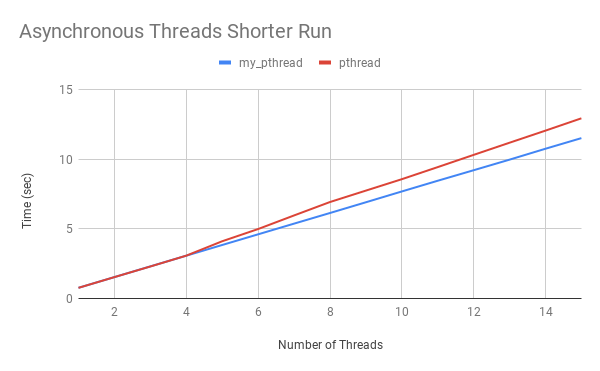
\includegraphics[width=\textwidth]{Asynchronous_Threads_Shorter_Run.png}
        \caption{Compares the time elapsed for each thread library to asynchronously run 1 to 15 threads, where each thread ran a shorter loop.}
        \label{async_short}
    \end{subfigure}
    \begin{subfigure}[b]{.49\textwidth}
        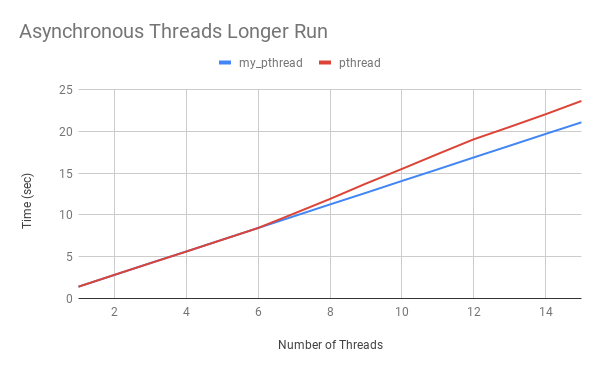
\includegraphics[width=\textwidth]{Asynchronous_Threads_Longer_Run.png}
        \caption{Compares the time elapsed for each thread library to asynchronously run 1 to 15 threads, where each thread ran a longer loop.}
        \label{async_long}
    \end{subfigure}
        \begin{subfigure}[b]{.49\textwidth}
        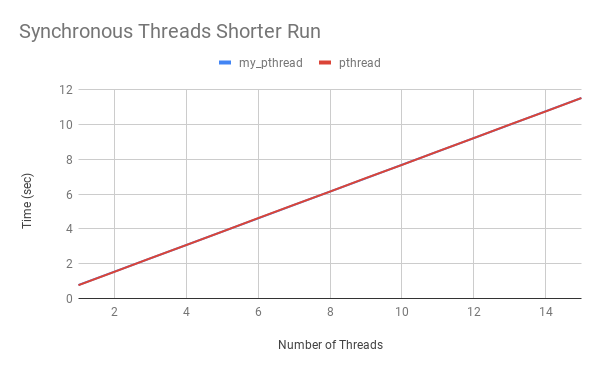
\includegraphics[width=\textwidth]{Synchronous_Threads_Shorter_Run.png}
        \caption{Compares the time elapsed for each thread library to synchronously run 1 to 15 threads, where each thread ran a shorter loop.}
        \label{sync_short}
    \end{subfigure}
    \begin{subfigure}[b]{.49\textwidth}
        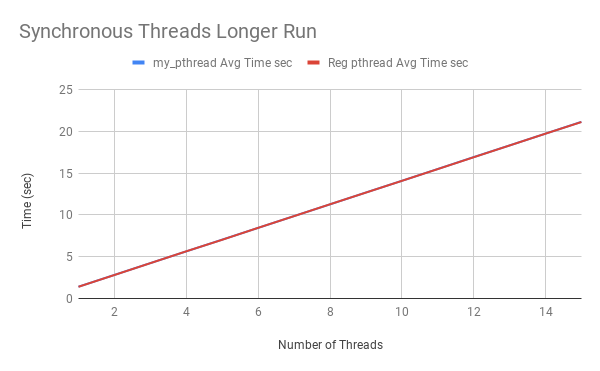
\includegraphics[width=\textwidth]{Synchronous_Threads_Longer_Run.png}
        \caption{Compares the time elapsed for each thread library to synchronously run 1 to 15 threads, where each thread ran a longer loop.}
        \label{sync_long}
    \end{subfigure}
\end{figure}

Comparing the libraries when threads were run asynchronously (\ref{async_long} and \ref{async_short}), we see that when the number of threads spawned is smaller the two libraries take the same amount of time, however as the number of threads increases, the POSIX library takes more time than our library. This trend is the same whether we ran the threads for a shorter duration or a longer duration. On the other hand, the libraries are quite comparable in terms of efficiency with synchronous thread execution (\ref{sync_short} and \ref{sync_long}). This is true for both threads that ran for a longer duration or a shorter duration. 
%% 

\section{Further Work}
In terms of further work, we could further optimize the scheduling mechanism. For example, each thread runs for 25 ms or a multiple of it before being swapped. We could play around with this value in an effort to ensure we find a sweet spot between first come first serve scheduling system and high overhead of too many context switches. Additionally, we decided to schedule a maintenance every second, however we might have been able to wait longer between maintaining our priority queue without starving any long running processes. By playing with how often we schedule maintenances, we could find a better balance of reducing the time spent maintaining the priority queue without starving long running threads. Likewise, other scheduling parameters such as number of queues, how much to decay and age a queue by could all be further fine tuned.
\end{document}

% List of tex snippets:
%   - tex-header (this)
%   - R      --> \mathbb{R}
%   - Z      --> \mathbb{Z}
%   - B      --> \mathcal{B}
%   - E      --> \mathcal{E}
%   - M      --> \mathcal{M}
%   - m      --> \mathfrak{m}({#1})
%   - normlp --> \norm{{#1}}_{L^{{#2}}}
